\subsubsection{Inner product}
\begin{frame}{Inner product}
    \begin{itemize}
            \item The dot product (also known as inner product) between two $n$-vectors $a$ and $b$ is defined  and denoted as the scalar:
            \begin{align}
                    a^Tb = a_1b_1 + a_2b_2 +  \cdots + a_n b_n
            \end{align}
            \item Alternative notations include: $(a, b)$ and $a\cdot b$. And we write it as: $(a, b)=a^Tb$ or $a\cdot b = a^Tb$.
            \item Illustration:
            \begin{align}
                    \begin{bmatrix}
                            1\\2\\3
                    \end{bmatrix}^T \begin{bmatrix}
                            1\\\frac{1}{2}\\-2
                    \end{bmatrix} = (1\times 1)+ (2\times \frac 1 2) + (3 \times -2) = -4
            \end{align}
    \end{itemize}  
\end{frame}

\begin{frame}{Key Properties}
\begin{itemize}
        \item Fundamental properties:
        \begin{itemize}
        \item Commutativity: $a^T b = b^T a$
        \item Scalar multiplication: $(\lambda a)^T b = \lambda (a^T b)$
        \item Distributivity: $(a + b) ^Tc = a^T c + b^T c$
        \item Zero vector: $0^T a = a^T 0 = 0$ for any vector $a$
\end{itemize}
\item Practical applications:
\begin{itemize}
        \item $e^T_i a = a_i$ (extracts the $i$-th component)
        \item $\boldsymbol{1}^T a = a_1 +a_2 + \cdots + a_n$ (computes sum of entries)
        \item $a^Ta = a_1^2 + \cdots + a_n^2$ (sum of squared entries)
\end{itemize}
\item \textbf{Note :} An Euclidean space is a vector space  with inner product.
\end{itemize}    
\end{frame}


\subsubsection{Norms, Distance and Angle}
\begin{frame}{Vector Norms}
\begin{itemize}
        \item The Euclidean norm of a vector $x$ is defined as:
        \begin{align}
                \Vert x \Vert = \sqrt{x_1^2 + x_2^2 + \cdots + x_n^2} = \sqrt{x^T x} \label{eq2,9}
        \end{align}
        \item For $n=1$, this simplifies to the absolute value.
        \item \textbf{Example:} For $x = \begin{bmatrix} 3 \\ 4 \end{bmatrix}$, the norm is:
        \begin{align*}
                \Vert x \Vert = \sqrt{3^2 + 4^2} = \sqrt{9 + 16} = \sqrt{25} = 5
        \end{align*}
        \item The norm is a measure of the distance from the origin to the point represented by the vector in a vector space.
\end{itemize}
\end{frame}

\begin{frame}{}
     \begin{figure}
            \begin{center}
        % Second diagram: Vector representation
        \begin{tikzpicture}
                % Axes
                \draw[->] (0,0) -- (3,0) node[below] {$x_1$};
                \draw[->] (0,0) -- (0,3) node[left] {$x_2$};
                % Vector
                \draw[->,blue,thick] (0,0) -- (2.5,2.5)  node[midway, right] {$\Vert x \Vert$};
                \draw[ blue] (2.5,2.5) node[right]{$x$};
        \end{tikzpicture}
         \hspace{1.5cm} % Space between the two figures
        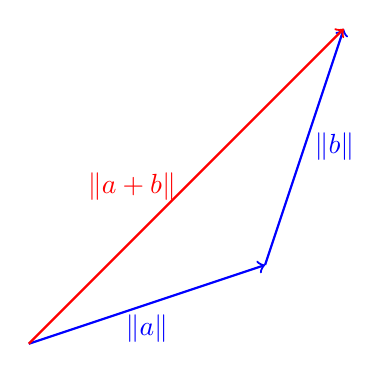
\begin{tikzpicture}
                % Draw grid
                % \draw[gray!50] (-1,-1) grid (5,4);
                
                % Define vectors
                \coordinate (O) at (0,0);
                \coordinate (A) at (3,1);
                \coordinate (B) at (1,3);
                \coordinate (C) at (4,4);
                
                % Draw vectors
                \draw[->, thick, blue] (O) -- (A) node[midway, below] {$\Vert a \Vert$};
                \draw[->, thick, blue] (A) -- (C) node[midway, right] {$\Vert b \Vert$};
                \draw[->, thick, red] (O) -- (C) node[midway, left] {$\Vert a + b \Vert$};
        \end{tikzpicture}
        \caption{(Left) Geometric representation of 2-vector norms. (Right) Triangle inequality visualization}
        \end{center}
 \end{figure}
\end{frame}

\begin{frame}
    \begin{itemize}
        \item The norm is also known as the \textbf{length} or \textbf{magnitude} of the vector.
        \item \textbf{Note :} There are other types of norms, such as the $L_1$  and $L_\infty$ norms, which are defined as:
        \begin{align}
        L_1 \;\text{norm :} \;\;\Vert x \Vert_1 = |x_1| + |x_2| + \cdots + |x_n|\\
        L_\infty \text{ norm:} \;\;\Vert x \Vert_\infty = \max(|x_1|, |x_2|, \ldots, |x_n|)
        \end{align}
   
        \item The Euclidean(also known as $L_2$ ) norm is the most commonly used norm. 
    \end{itemize}
\end{frame}
\begin{frame}
    \begin{itemize}
        \item Visual comparison of different norms for the same vector:
        \begin{figure}
            \begin{center}
                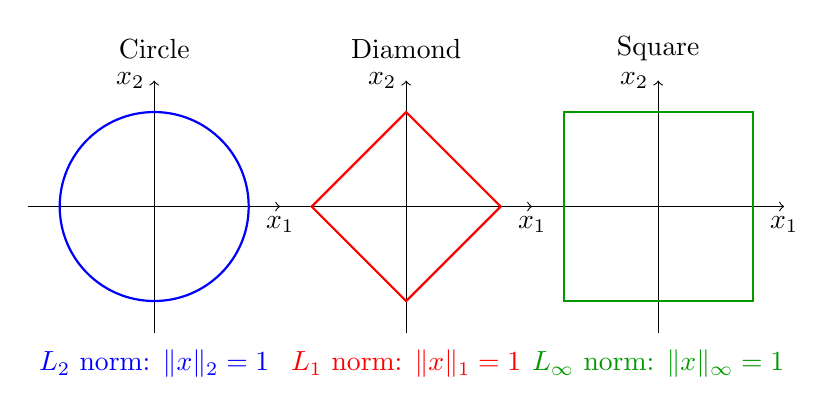
\begin{tikzpicture}[scale=0.8]
                    % L2 norm (circle)
                    \begin{scope}[xshift=-4cm]
                        \draw[->] (-2,0) -- (2,0) node[below] {$x_1$};
                        \draw[->] (0,-2) -- (0,2) node[left] {$x_2$};
                        \draw[blue, thick] (0,0) circle (1.5);
                        \node[blue] at (0,-2.5) {$L_2$ norm: $\|x\|_2 = 1$};
                        \node at (0,2.5) {Circle};
                    \end{scope}
                    
                    % L1 norm (diamond)
                    \begin{scope}
                        \draw[->] (-2,0) -- (2,0) node[below] {$x_1$};
                        \draw[->] (0,-2) -- (0,2) node[left] {$x_2$};
                        \draw[red, thick] (1.5,0) -- (0,1.5) -- (-1.5,0) -- (0,-1.5) -- cycle;
                        \node[red] at (0,-2.5) {$L_1$ norm: $\|x\|_1 = 1$};
                        \node at (0,2.5) {Diamond};
                    \end{scope}
                    
                    % L∞ norm (square)
                    \begin{scope}[xshift=4cm]
                        \draw[->] (-2,0) -- (2,0) node[below] {$x_1$};
                        \draw[->] (0,-2) -- (0,2) node[left] {$x_2$};
                        \draw[green!60!black, thick] (-1.5,-1.5) rectangle (1.5,1.5);
                        \node[green!60!black] at (0,-2.5) {$L_\infty$ norm: $\|x\|_\infty = 1$};
                        \node at (0,2.5) {Square};
                    \end{scope}
                \end{tikzpicture}
            \end{center}
            \caption{Unit balls for different norms in 2D space}
        \end{figure}
        \item Each shape represents all vectors with norm equal to 1 under the respective norm definition.
    \end{itemize}
\end{frame}



\begin{frame}{Norm Properties}
All norms for $n$-vectors $x$ and $y$ and scalar $\lambda$ must satisfy these axioms:
\begin{itemize}
    \item \textbf{Scaling property}: $\Vert \lambda x \Vert = \vert \lambda \vert \Vert x \Vert$
    \item \textbf{Trinagual inequality}: $ \Vert x+ y \Vert \leq \Vert x \Vert + \Vert y \Vert$
    \item \textbf{Non-negativity}: $\Vert x \Vert \geq 0$
    \item \textbf{Zero condition}: $\Vert x \Vert = 0$ if and only if $x = 0$
\end{itemize}
\textbf{Note:} That is, for a function to be a norm, it must satisfy these properties.\\

\end{frame}

\begin{frame}
\textbf{Exercise}: Verify these properties hold for the $L_1$, $L_2$, and $L_\infty$ norms.\\
\textbf{Exercice:} Does the function $\Vert x \Vert = \sqrt{x_1^2 + x_2^2 + 1}$ satisfy the norm properties? Why or why not?
\end{frame}



\begin{frame}{Norm of Block Vectors}
\begin{itemize}
    \item Consider block vector formed by concatenating vectors $a$, $b$, and $c$:
    \item The squared norm satisfies:
    \begin{align}
        \Vert (a,b,c) \Vert ^2 = a^Ta + b^T b + c^Tc = \Vert a \Vert ^2 + \Vert b \Vert ^2 + \Vert c \Vert ^2
    \end{align}
    \item Therefore, the norm of the block vector is:
    \begin{align}
        \Vert (a, b, c) \Vert = \sqrt{\Vert a \Vert ^2 + \Vert b \Vert ^2 + \Vert c \Vert ^2}
    \end{align}
    \item This property extends to any number of block components.
\end{itemize}
\end{frame}

\begin{frame}{Euclidean Distance Between Vectors}
\begin{itemize}
    \item The Euclidean distance between two $n$-vectors $a$ and $b$ is defined as:
    \begin{align}
        \text{dist}(a, b) = \Vert a - b\Vert = \sqrt{(a_1-b_1)^2 + \cdots + (a_n-b_n)^2}
    \end{align}
    \item Geometric interpretation in 2D space:
    \begin{center}
    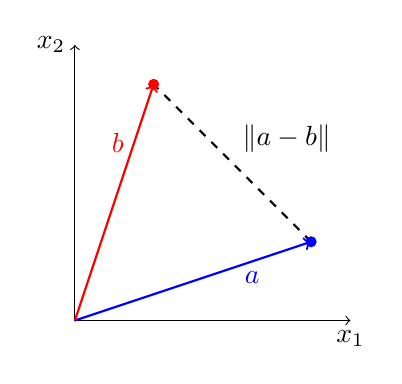
\begin{tikzpicture}
        % Define vectors
        \coordinate (O) at (0,0);
        \coordinate (A) at (3,1);
        \coordinate (B) at (1,3);
        
        % Draw axes
        \draw[->] (0,0) -- (3.5,0) node[below] {$x_1$};
        \draw[->] (0,0) -- (0,3.5) node[left] {$x_2$};
        
        % Draw vectors
        \draw[->, thick, blue] (O) -- (A) node[near end, below] {$a$};
        \draw[->, thick, red] (O) -- (B) node[near end, left] {$b$};
        
        % Draw distance between vectors
        \draw[dashed, black, thick] (A) -- (B) node[midway, above right] {$\|a - b\|$};
        
        % Add points
        \fill[blue] (A) circle (2pt);
        \fill[red] (B) circle (2pt);
    \end{tikzpicture}
    \end{center}
\end{itemize}
\end{frame}

\begin{frame}
    \begin{itemize}
        \item The distance is zero if and only if $a = b$.
        \item The distance satisfies the \textbf{triangle inequality}:
        \begin{align}
            \text{dist}(a, b) + \text{dist}(b, c) \geq \text{dist}(a, c)
        \end{align}
        \item The distance can also be generalized to other norms, such as $L_1$ and $L_\infty$:
        \begin{align}
            \text{dist}_1(a, b) = \Vert a - b \Vert_1 = |a_1 - b_1| + |a_2 - b_2| + \cdots + |a_n - b_n|\\
            \text{dist}_\infty(a, b) = \Vert a - b \Vert_\infty = \max(|a_1 - b_1|, |a_2 - b_2|, \ldots, |a_n - b_n|)
        \end{align}
    \end{itemize}
\end{frame}
\begin{frame}
\begin{itemize}
    \item Example: For vectors $a = \begin{bmatrix} 3 \\ 4 \end{bmatrix}$ and $b = \begin{bmatrix} 1 \\ 2 \end{bmatrix}$:
    \begin{align*}
        \text{dist}(a, b) = \sqrt{(3-1)^2 + (4-2)^2} = \sqrt{2^2 + 2^2} = \sqrt{4 + 4} = \sqrt{8} = 2\sqrt{2}
    \end{align*}
    \item The distance can be interpreted as the length of the line segment connecting points $a$ and $b$ in 2D space. 
\end{itemize}
\end{frame}

\begin{frame}{Statistical Properties Using Inner Products and Norms}
We can compute  statstic measures of vector $x$ in terms of its norm:
\begin{itemize}
    \item For an $n$-vector $x$, the mean can be expressed using inner products:
    \begin{align}
        \overline{x} = \frac{1}{n} \boldsymbol{1}^T x
    \end{align}
    \item The centered (de-meaned) vector is obtained by:
    \begin{align*}
        \tilde{x} = x - \overline{x} \boldsymbol{1}
    \end{align*}
    \item The standard deviation can be computed using the norm:
    \begin{align*}
        \text{std}(x) = \frac{\Vert \tilde{x} \Vert}{\sqrt{n}} = \frac{\Vert x - \overline{x} \boldsymbol{1} \Vert}{\sqrt{n}}
    \end{align*}
\end{itemize}
\end{frame}

\begin{frame}{}
\begin{itemize}
    \item The mean square value of vector $x$ is defined as:
    \begin{align}
        \text{MSV}(x) = \frac{x_1^2 + \cdots + x_n^2 }{n} = \frac{\Vert x \Vert^2 }{n}
    \end{align}
    \item The root mean square (RMS) value of vector $x$ is:
    \begin{align}
        \text{RMS}(x) = \sqrt{ \frac{x_1^2 + \cdots + x_n^2 }{n}} = \frac{\Vert x \Vert}{\sqrt{n}}
    \end{align}
\end{itemize}
\end{frame}
\begin{frame}
\begin{itemize}
    \item The variance of vector $x$ is defined as:
    \begin{align}
        \text{Var}(x) = \frac{1}{n} \Vert x - \overline{x} \boldsymbol{1} \Vert^2 = \frac{1}{n} (x - \overline{x} \boldsymbol{1})^T (x - \overline{x} \boldsymbol{1})
    \end{align}
    \item The covariance matrix of vector $x$ is given by:
    \begin{align}
        C(x) = \frac{1}{n} (x - \overline{x} \boldsymbol{1})(x - \overline{x} \boldsymbol{1})^T
    \end{align}
    \item The covariance matrix captures the variance and covariance of the components of vector $x$.
\end{itemize}
\end{frame}


\subsubsection{Some Norms Inequalities}
\begin{frame}{Some Norms Inequalities}
\begin{block}{\textbf{Cauchy-Schwarz Inequality}}
    For any $n$-vectors $a$ and $b$, the following inequality holds:
    \begin{align}
        |a^T b| \leq \|a\| \|b\|
    \end{align}
    This fundamental result is known as the \textbf{Cauchy-Schwarz inequality}.
\end{block}
\textbf{Proof:}
\begin{itemize}
    \item Consider the vector $c = a - \lambda b$ for some scalar $\lambda$.
    \item The norm of $c$ must be non-negative:
    \begin{align*}
        \|c\|^2 = (a - \lambda b)^T (a - \lambda b) \geq 0
    \end{align*}
\end{itemize}
\end{frame}

\begin{frame}
    \begin{itemize}
        \item Expanding this gives:
    \begin{align*}
        a^T a - 2\lambda a^T b + \lambda^2 b^T b \geq 0
    \end{align*}
    \item This is a quadratic in $\lambda$, which must have non-negative discriminant:
    \begin{align*}
        (a^T b)^2 - a^T a b^T b \geq 0
    \end{align*}
    \item Rearranging yields the Cauchy-Schwarz inequality:
    \begin{align*}
        |a^T b|^2 \leq (a^T a)(b^T b)
    \end{align*}
    \item Taking square roots gives:
    \begin{align*}
        |a^T b| \leq \|a\| \|b\|
    \end{align*}
    \end{itemize}
\end{frame}
  
\begin{frame}
    \textbf{Exercise:} Use the Cauchy-Schwarz inequality to demonstrate that the triangle inequality holds for vector norms, i.e., show that:
    \begin{align*}
        \|a + b\| \leq \|a\| + \|b\|
    \end{align*}
\end{frame}
\begin{frame}
\begin{block}{\textbf{Minkowski Inequality}}
    For any $n$-vectors $a$ and $b$, and for $p \geq 1$, the following holds:
    \begin{align}
        \|a + b\|_p \leq \|a\|_p + \|b\|_p
    \end{align}
    This is known as the \textbf{Minkowski inequality}. 
\end{block}
\textbf{Proof: }
\begin{itemize}
    \item Consider the $p$-norm defined as:
    \begin{align*}
        \|x\|_p = (|x_1|^p + |x_2|^p + \cdots + |x_n|^p)^{1/p}
    \end{align*}
    \item The Minkowski inequality states that the $p$-norm satisfies the triangle inequality.
    \item This can be shown using the Cauchy-Schwarz inequality for $p$-norms.
\end{itemize}
\end{frame}
\begin{frame}
    \begin{itemize}
        \item An other way to show  the Minkowsky's inequality is  to  use the convexity of the function $f(x) = |x|^p$ for $p \geq 1$.
        \item The function $f(x)$ is convex, because its second derivative is non-negative:
        \begin{align*}
            f''(x) = p(p-1)|x|^{p-2}
        \end{align*}
        \item Convex functions satisfy the Jensen's inequality:
        \begin{align*}
            f(\lambda x + (1 - \lambda) y) \leq \lambda f(x) + (1 - \lambda) f(y)
        \end{align*}    

     for all $\lambda \in [0, 1]$.
    \end{itemize}
\end{frame}

\begin{frame}
    \begin{itemize}
        \item Applying this to the $p$-norm gives:
        \begin{align*}
            \|a + b\|_p^p = (|a_1 + b_1|^p + |a_2 + b_2|^p + \cdots + |a_n + b_n|^p) \leq (|a_1|^p + |b_1|^p + \cdots + |a_n + b_n|^p)
        \end{align*}
        \item Taking the $p$-th root yields the Minkowski inequality:
        \begin{align*}
            \|a + b\|_p \leq \|a\|_p + \|b\|_p
        \end{align*} 
    \end{itemize}
\end{frame}

\begin{frame}
    \begin{block}{\textbf{Holder's Inequality}}
        For any $n$-vectors $a$ and $b$ and for any $p, q > 1$ such that $\frac{1}{p} + \frac{1}{q} = 1$, the following holds:
        \begin{align}
            |a^T b| \leq \|a\|_p \|b\|_q
        \end{align}
        This is known as \textbf{Hölder's inequality}.
    \end{block}
    \textbf{Proof: Exercice}
\end{frame}


% ------------ Angles Between Vectors ------------
\subsubsection{Angles Between Vectors}

\begin{frame}{Angle Between Vectors}
\begin{itemize}
    \item Two vectors sharing a common origin define an angle between them.
    \begin{center}
    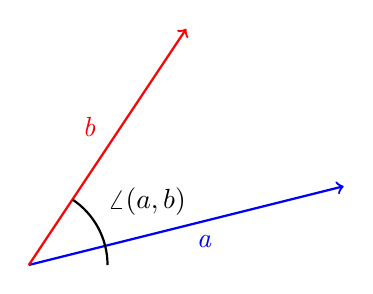
\begin{tikzpicture}
        % Define vectors
        \coordinate (O) at (0,0);
        \coordinate (A) at (4,1);
        \coordinate (B) at (2,3);
        
        % Draw vectors
        \draw[->, thick, blue] (O) -- (A) node[midway, below right] {\textit{a}};
        \draw[->, thick, red] (O) -- (B) node[midway, above left] {\textit{b}};
        
        % Draw angle arc
        \draw[thick] (1,0) arc (0:56:1);
        \node at (1.5,0.8){$\angle(a,b)$};
    \end{tikzpicture}
\end{center}
    \item The angle between two vectors $a$ and $b$ is given by:
    \begin{align}
        \angle(a, b) = \arccos \left(\frac{\langle a, b \rangle}{\Vert a \Vert \times \Vert b \Vert} \right) \label{eq2,22}
    \end{align}
\end{itemize}
\end{frame}
\begin{frame}
    \begin{itemize}
        \item The existence of the angle is guaranteed by the Cauchy-Schwarz inequality:
        \begin{align}
            |\langle a, b \rangle| \leq \Vert a \Vert \Vert b \Vert
        \end{align}
        \item For non-zero vectors $a$ and $b$, we can normalize the inner product:
        \begin{align*}
            -1 \leq \frac{\langle a, b \rangle }{\Vert a \Vert \Vert b \Vert} \leq 1
        \end{align*}
        \item Since $\arccos$ is defined on the interval $[-1, 1]$ and maps bijectively to $[0, \pi]$, the angle $\angle(a, b)$ is well-defined.
        \item For more details, refer to the blog post  \textit{\href{https://www.jmabiala.com/blog/continuous_inverse_theorem}{continuous inverse theorem}}.
    \end{itemize}
\end{frame}


\begin{frame}{Properties of Angles}
\begin{itemize}
    \item The angle is always between $0$ and $\pi$ radians (or $0$ and $180^\circ$).
    \item If the angle is $0$, the vectors are in the same direction.
    \item If the angle is $\pi$, the vectors are    in opposite directions. 
    \item If the angle is $\frac{\pi}{2}$, the vectors are orthogonal (perpendicular).
    \item The angle can be computed using the inner product:
\end{itemize}
\end{frame}


\begin{frame}{}
\begin{itemize}
    \item From equation \ref{eq2,22}, we can express the dot product of vectors $a$ and $b$ as:
    \begin{align}
        a^T b = \|a\| \|b\| \cos(\angle(a, b))
    \end{align}
    \item This gives us insight into the sign of the dot product:
    \begin{itemize}
        \item $a^T b > 0$ when $\angle(a, b) < \frac{\pi}{2}$ (acute angle)
        \item $a^T b = 0$ when $\angle(a, b) = \frac{\pi}{2}$ (orthogonal vectors)
        \item $a^T b < 0$ when $\angle(a, b) > \frac{\pi}{2}$ (obtuse angle)
    \end{itemize}
\end{itemize}
\end{frame}

\begin{frame}
    \begin{figure}
        \begin{center}
        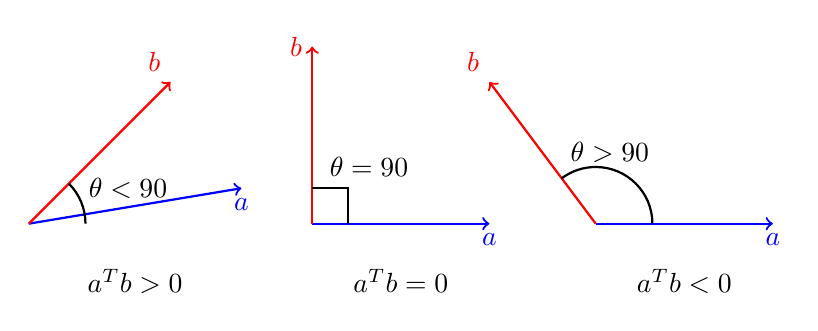
\begin{tikzpicture}[scale=0.9]
            % Acute angle case
            \begin{scope}[xshift=-4cm]
                \coordinate (O) at (0,0);
                \coordinate (A) at (3,0.5);
                \coordinate (B) at (2,2);
                
                \draw[->, thick, blue] (O) -- (A) node[below] {$a$};
                \draw[->, thick, red] (O) -- (B) node[above left] {$b$};
                \draw[thick] (0.8,0) arc (0:45:0.8);
                \node at (1.4,0.5) {$\theta < 90$};
                \node[below] at (1.5,-0.5) {$a^T b > 0$};
            \end{scope}
            
            % Right angle case
            \begin{scope}
                \coordinate (O) at (0,0);
                \coordinate (A) at (2.5,0);
                \coordinate (B) at (0,2.5);
                
                \draw[->, thick, blue] (O) -- (A) node[below] {$a$};
                \draw[->, thick, red] (O) -- (B) node[left] {$b$};
                \draw[thick] (0.5,0) -- (0.5,0.5) -- (0,0.5);
                \node at (0.8,0.8) {$\theta = 90$};
                \node[below] at (1.25,-0.5) {$a^T b = 0$};
            \end{scope}
            
            % Obtuse angle case
            \begin{scope}[xshift=4cm]
                \coordinate (O) at (0,0);
                \coordinate (A) at (2.5,0);
                \coordinate (B) at (-1.5,2);
                
                \draw[->, thick, blue] (O) -- (A) node[below] {$a$};
                \draw[->, thick, red] (O) -- (B) node[above left] {$b$};
                \draw[thick] (0.8,0) arc (0:127:0.8);
                \node at (0.2,1) {$\theta > 90$};
                \node[below] at (1.25,-0.5) {$a^T b < 0$};
            \end{scope}
        \end{tikzpicture}
        \caption{Relationship between dot product sign and angle between vectors}
        \end{center}
    \end{figure}
\end{frame}

\begin{frame}{Example}
    \begin{itemize}
        \item Consider vectors $a = \begin{bmatrix} 1 \\ 2 \end{bmatrix}$ and $b = \begin{bmatrix} 3 \\ 4 \end{bmatrix}$.
        \item Compute the angle between them:
        \begin{align*}
            a^T b = 1 \cdot 3 + 2 \cdot 4 = 3 + 8 = 11\\
            \|a\| = \sqrt{1^2 + 2^2} = \sqrt{5}\\
            \|b\| = \sqrt{3^2 + 4^2} = \sqrt{25} = 5
        \end{align*}
        \item The angle is:
        \begin{align*}
            \angle(a, b) = \arccos\left(\frac{11}{\sqrt{5} \cdot 5}\right) = \arccos\left(\frac{11}{5\sqrt{5}}\right)
        \end{align*}
    \end{itemize}
\end{frame}
\begin{frame}
    \textbf{Example:} Consider vectors $a = \begin{bmatrix} 3 \\ 4 \\ 0 \end{bmatrix}$ and $b = \begin{bmatrix} 4 \\ -3 \\ 5 \end{bmatrix}$.
    \begin{itemize}
        \item Compute the angle between them:
        \begin{align*}
            a^T b = 3 \cdot 4 + 4 \cdot (-3) + 0 \cdot 5 = 12 - 12 + 0 = 0\\
            \|a\| = \sqrt{3^2 + 4^2 + 0^2} = \sqrt{9 + 16} = 5\\
            \|b\| = \sqrt{4^2 + (-3)^2 + 5^2} = \sqrt{16 + 9 + 25} = \sqrt{50} = 5\sqrt{2}
        \end{align*}
        \item The angle is:
        \begin{align*}
            \angle(a, b) = \arccos\left(\frac{0}{5 \cdot 5\sqrt{2}}\right) = \arccos(0) = \frac{\pi}{2}
        \end{align*}
    \end{itemize}
\end{frame}

\begin{frame}
    \begin{itemize}
        \item \textbf{Exercise} (Pythagorean theorem): Prove that for any $n$-vectors $a$ and $b$:
    \begin{align}
        \|a + b\|^2 = \|a\|^2 + \|b\|^2 \quad \text{if and only if} \quad \angle(a, b) = \frac{\pi}{2}
    \end{align}
    \item \textbf{Exercise}: Determine the angles between the standard unit vectors $e_1$, $e_2$, and $e_3$ in $\mathbb{R}^3$.
    \end{itemize}
\end{frame}


% ---------------------- Orthogonality ----------------------
\subsubsection{Orthogonality}
\begin{frame}{Orthogonal Vectors and Orthogonality}
\begin{itemize}
\item \textbf{Orthonanility:} Two $n$-vectors $a$ and $b$ are orthogonal, denoted $a \perp b$, if their inner product is zero:
\begin{align}
    a^T b = a_1 b_1 + a_2 b_2 + \cdots + a_n b_n = 0
\end{align}
\item \textbf{Example:} The standard unit vectors $e_1$ and $e_2$ are orthogonal. For $n=3$:
\begin{align*}
    e_1^T e_2 = \begin{bmatrix} 1 \\ 0 \\ 0 \end{bmatrix}^T \begin{bmatrix} 0 \\ 1 \\ 0 \end{bmatrix} = (1)(0) + (0)(1) + (0)(0) = 0
\end{align*}
\end{itemize}
\end{frame}


\begin{frame}{}
\begin{itemize}
    \item \textbf{Mutual orthogonaity:} A set of vectors $a_1, \ldots, a_k$ are called \textbf{mutually orthogonal} if $a_i \perp a_j$ for all $i \neq j$.
    \item The standard unit vectors $e_1, \ldots, e_n$ form a mutually orthogonal set, satisfying:
    \begin{align}
        e_i^T e_j = \delta_{ij} = \begin{cases}
             1 & \text{if } i = j \\
             0 & \text{if } i \neq j
        \end{cases}
    \end{align}
    \item The quantity $\delta_{ij}$ is called the \textbf{Kronecker delta}.
\end{itemize}
\end{frame}
\begin{frame}
    \begin{figure}
        \begin{center}
        \begin{tikzpicture}
        % Define standard orthogonal vectors
        \coordinate (O) at (0,0);
        \coordinate (A1) at (3,0);
        \coordinate (B1) at (0,3);
        
        % Draw first set of orthogonal vectors
        \draw[->, thick, blue] (O) -- (A1) node[midway, below] {\textit{u}};
        \draw[->, thick, red] (O) -- (B1) node[midway, left] {\textit{v}};
        
        % Draw right angle marker
        \draw[thick] (1,0) -- (1,1) -- (0,1);
        
        % Define second rotated orthogonal vectors
        \coordinate (OO) at (6,0);  % Shifted origin
        \coordinate (A2) at (7,2);  % Rotated u
        \coordinate (B2) at (4,1);  % Rotated v, now orthogonal to u
        
        % Draw second set of orthogonal vectors
        \draw[->, thick, cyan] (OO) -- (A2) node[midway, below right] {\textit{u}};
        \draw[->, thick, magenta] (OO) -- (B2) node[midway, above left] {\textit{v}};
        
        % Draw right angle marker for rotated vectors
        % \draw[thick] (6.4,0.4) -- (6.2,0.8) -- (5.8,0.6);
    \end{tikzpicture}
    \end{center}
    \caption{Examples of orthogonal vector pairs in $\mathbb{R}^2$}
    \end{figure}
\end{frame}

\begin{frame}
    \begin{itemize}
        \item \textbf{Orthonormality:} A set of vectors  $a_1, \ldots, a_k$ are \textbf{orthonormal} if they are mutually orthogonal and each vector has unit norm:
        \begin{align}
            \|a_i\| = 1 \quad \text{for all } i
        \end{align}
        \item The standard unit vectors $e_1, \ldots, e_n$ form an orthonormal set:
        \begin{align}
            \|e_i\| = 1 \quad \text{and} \quad e_i^T e_j = \delta_{ij} \quad \text{for all } i, j
        \end{align}
    \end{itemize}
\end{frame}

\begin{frame}
    \textbf{Exercice:} Show that  orthogonal vectors are linearly independent.
\end{frame}

\begin{frame}
\begin{block}{\textbf{Parseval's Identity}}
    For any $n$-vector $x = (x_1, x_2, \ldots, x_n) \in \mathbb{R}^n$ and any orthonormal basis $\{u_1, u_2, \ldots, u_n\}$, where $\|u_i\| = 1$ and $u_i^T u_j = \delta_{ij}$, the squared Euclidean norm satisfies:
    \begin{align}
        \|x\|_2^2 = \langle x, x \rangle = \sum_{i=1}^n \vert ( x, u_i )\vert ^2 = \sum_{i=1}^n (x^T u_i)^2
    \end{align}
    where $( \cdot, \cdot )$ denotes the standard inner product on $\mathbb{R}^n$. 
\end{block}
\textbf{Note:} This shows that the squared norm of a vector is preserved under any orthonormal basis representation.
\end{frame}


\begin{frame}{Orthonormal Expansion}
\begin{itemize}
    \item If $\{a_1, a_2, \ldots, a_n\}$ forms an orthonormal basis for $\mathbb{R}^n$, then any vector $x \in \mathbb{R}^n$ can be uniquely expressed as:
    \begin{align}
        x = (a_1^T x)a_1 + (a_2^T x)a_2 + \cdots + (a_n^T x)a_n = \sum_{i=1}^n (a_i^T x)a_i \label{eq2,39}
    \end{align}
    \item This representation is called the \textbf{orthonormal expansion} of $x$ with respect to the orthonormal basis $\{a_1, a_2, \ldots, a_n\}$.
    \item The coefficients $(a_i^T x)$ represent the projections of $x$ onto each basis vector $a_i$.
\end{itemize}
\end{frame}

\begin{frame}
    \textbf{Exercice:} Prove Parseval's identity by showing that the inner product of $x$ with each basis vector $u_i$ gives the projection of $x$ onto $u_i$, and that the sum of the squares of these projections equals the squared norm of $x$.\\
    \textbf{Exercise:} Prove this expansion \ref{eq2,39} by showing that the right-hand side equals $x$ using the orthonormality properties.
\end{frame}



\begin{frame}{Gram-Schmidt (orthogonalization) algorithm}
    \begin{itemize}
        \item An algorithm to construct orthogonal vectors from any vectors.
    \item \textbf{Given $k$ vectors of dimension $n$, $a_1,\ldots,a_k$}
    \item The $G-S$ algorithm generates orthonormal vectors $q_1, q_2, \ldots, q_k$ as follows:
    \begin{align*}
        q_1 & = a_1\\
        q_2 & = a_2 - \frac{a_2^Tq_1}{\Vert q_1 \Vert^2}q_1\\
      \vdots \;\; & = \; \vdots \\
        q_k & = a_k - \sum_{i=1}^{k-1} \frac{a_k^Tq_i}{\Vert q_i \Vert^2}q_i
    \end{align*}
    \end{itemize}
\end{frame}

\begin{frame}
    \begin{itemize}
        \item \textbf{Gram-Schmidt Algorithm:}
        \begin{enumerate}
            \item \textbf{Input:} Linearly independent vectors $a_1, a_2, \ldots, a_k \in \mathbb{R}^n$
            \item \textbf{Output:} Orthonormal vectors $q_1, q_2, \ldots, q_k \in \mathbb{R}^n$
            \item \textbf{For} $i = 1$ to $k$:
            \begin{itemize}
                \item Set $\tilde{q}_i \leftarrow a_i$
                \item \textbf{For} $j = 1$ to $i-1$: $\tilde{q}_i \leftarrow \tilde{q}_i - (a_i^T q_j) q_j$
                \item $q_i \leftarrow \frac{\tilde{q}_i}{\|\tilde{q}_i\|}$
            \end{itemize}
        \end{enumerate}
        \item The algorithm produces orthonormal vectors where $q_i^T q_j = \delta_{ij}$.
         \item The newly obtained vectors $q_1, \ldots, q_k$ are orthonormal. (Proof: exercise. Hint: induction).
        \item \textbf{Complexity:} $O(kn^2)$ operations for $k$ vectors of dimension $n$.
    \end{itemize}
\end{frame}

\begin{frame}{Example: Gram-Schmidt Algorithm}
\textbf{Example:} Let's consider the vectors 
\begin{align*}
    a_1 = \begin{bmatrix} 1 \\ 1 \\ 1 \end{bmatrix}, \quad 
    a_2 = \begin{bmatrix} 1 \\ 0 \\ 1 \end{bmatrix}, \quad 
    a_3 = \begin{bmatrix} 1 \\ 1 \\ 0 \end{bmatrix}
\end{align*}

\begin{itemize}
    \item These vectors are not orthogonal (verify by computing dot products).
    \item \textbf{Step 1:} $q_1 = \frac{a_1}{\|a_1\|} = \frac{1}{\sqrt{3}} \begin{bmatrix} 1 \\ 1 \\ 1 \end{bmatrix}$
\end{itemize}
\end{frame}
\begin{frame}
    \begin{itemize}
       \item \textbf{Step 2:} Orthogonalize $a_2$ against $q_1$:
    \begin{align*}
        \tilde{q}_2 &= a_2 - (a_2^T q_1) q_1 = \begin{bmatrix} 1 \\ 0 \\ 1 \end{bmatrix} - \frac{2}{\sqrt{3}} \cdot \frac{1}{\sqrt{3}} \begin{bmatrix} 1 \\ 1 \\ 1 \end{bmatrix} \\
        &= \begin{bmatrix} 1 \\ 0 \\ 1 \end{bmatrix} - \frac{2}{3} \begin{bmatrix} 1 \\ 1 \\ 1 \end{bmatrix} = \begin{bmatrix} 1/3 \\ -2/3 \\ 1/3 \end{bmatrix}
    \end{align*}
    Then normalize: $q_2 = \frac{\tilde{q}_2}{\|\tilde{q}_2\|}$
    \end{itemize}
\end{frame}

\begin{frame}
    \begin{itemize}
        \item \textbf{Step 3:} Orthogonalize $a_3$ against $q_1$ and $q_2$:
        \begin{align*}
            \tilde{q}_3 &= a_3 - (a_3^T q_1) q_1 - (a_3^T q_2) q_2
        \end{align*}
        Compute the projections and normalize to get $q_3$.
        
        \item The final orthonormal vectors are:
        \begin{align*}
            q_1, q_2, q_3
        \end{align*}
        
        \item \textbf{Verification:} Let us check that $q_i^T q_j = \delta_{ij}$ for all $i, j$.
    \end{itemize}
\end{frame}

\begin{frame}
    \begin{itemize}
        \item Compute the inner products:
        \begin{align*}
            q_1^T q_2 &= \frac{1}{\sqrt{3}} \cdot \frac{1}{\sqrt{3}} \left(1 \cdot 1 + 1 \cdot 0 + 1 \cdot 1\right) = \frac{1}{3} \cdot 2 = \frac{2}{3} \\
            q_1^T q_3 &= \frac{1}{\sqrt{3}} \cdot \frac{1}{\sqrt{3}} \left(1 \cdot 1 + 1 \cdot 1 + 1 \cdot 0\right) = \frac{1}{3} \cdot 2 = \frac{2}{3} \\
            q_2^T q_3 &= \frac{1}{\sqrt{3}} \cdot \frac{1}{\sqrt{3}} \left(\frac{1}{3} \cdot 1 + \left(-\frac{2}{3}\right) \cdot 1 + \frac{1}{3} \cdot 0\right) = \frac{1}{3} \cdot 0 = 0
        \end{align*}
        \item Since $q_1^T q_2 = 0$, $q_1^T q_3 = 0$, and $q_2^T q_3 = 0$, the vectors are orthogonal.
        \item Normalize each vector to ensure they have unit norm:
        \begin{align*}
            \|q_1\| = \|q_2\| = \|q_3\| = 1
        \end{align*}
        \item Therefore, the vectors $q_1, q_2, q_3$ form an orthonormal set.
    \end{itemize}
\end{frame}



